	\chapter{Einleitung}
	\section{Motivation}
	Menschen sind schon immer fasziniert von der Frage nach ihrer eigenen Herkunft und der des Universums in dem sie Leben. Eine Facette dieser Frage ist der Wunsch, ein besseres Verständnis des kosmischen Zyklus von der Entstehung und dem Vergehen von Sternen zu erlangen. Dieses Thema ist insbesondere deshalb interessant, weil mit ihm die Entstehung von Planetensystemen verknüpft ist und es somit unsere eigene Herkunft berührt.
	
	In der Astrophysik lassen sich zwei Wege einschlagen um sich diesem Ver\-ständ\-nis zu nähern. Der eine Weg führt über die Beobachtung der Sternentstehungsgebiete, in denen nebeneinander verschiedene Entwicklungsstadien der Sternentstehung beobachtet werden können --- von Molekülwolken über Globulen, junge stellare Objekte (YSOs) mit protoplanetarer Scheibe, Vorhauptreihensterne bis hin zu Hauptreihensternen.
	%\begin{wrapfigure}{l}{0.382\textwidth}
	%	\centering
	%	\vspace{-1em}
	%	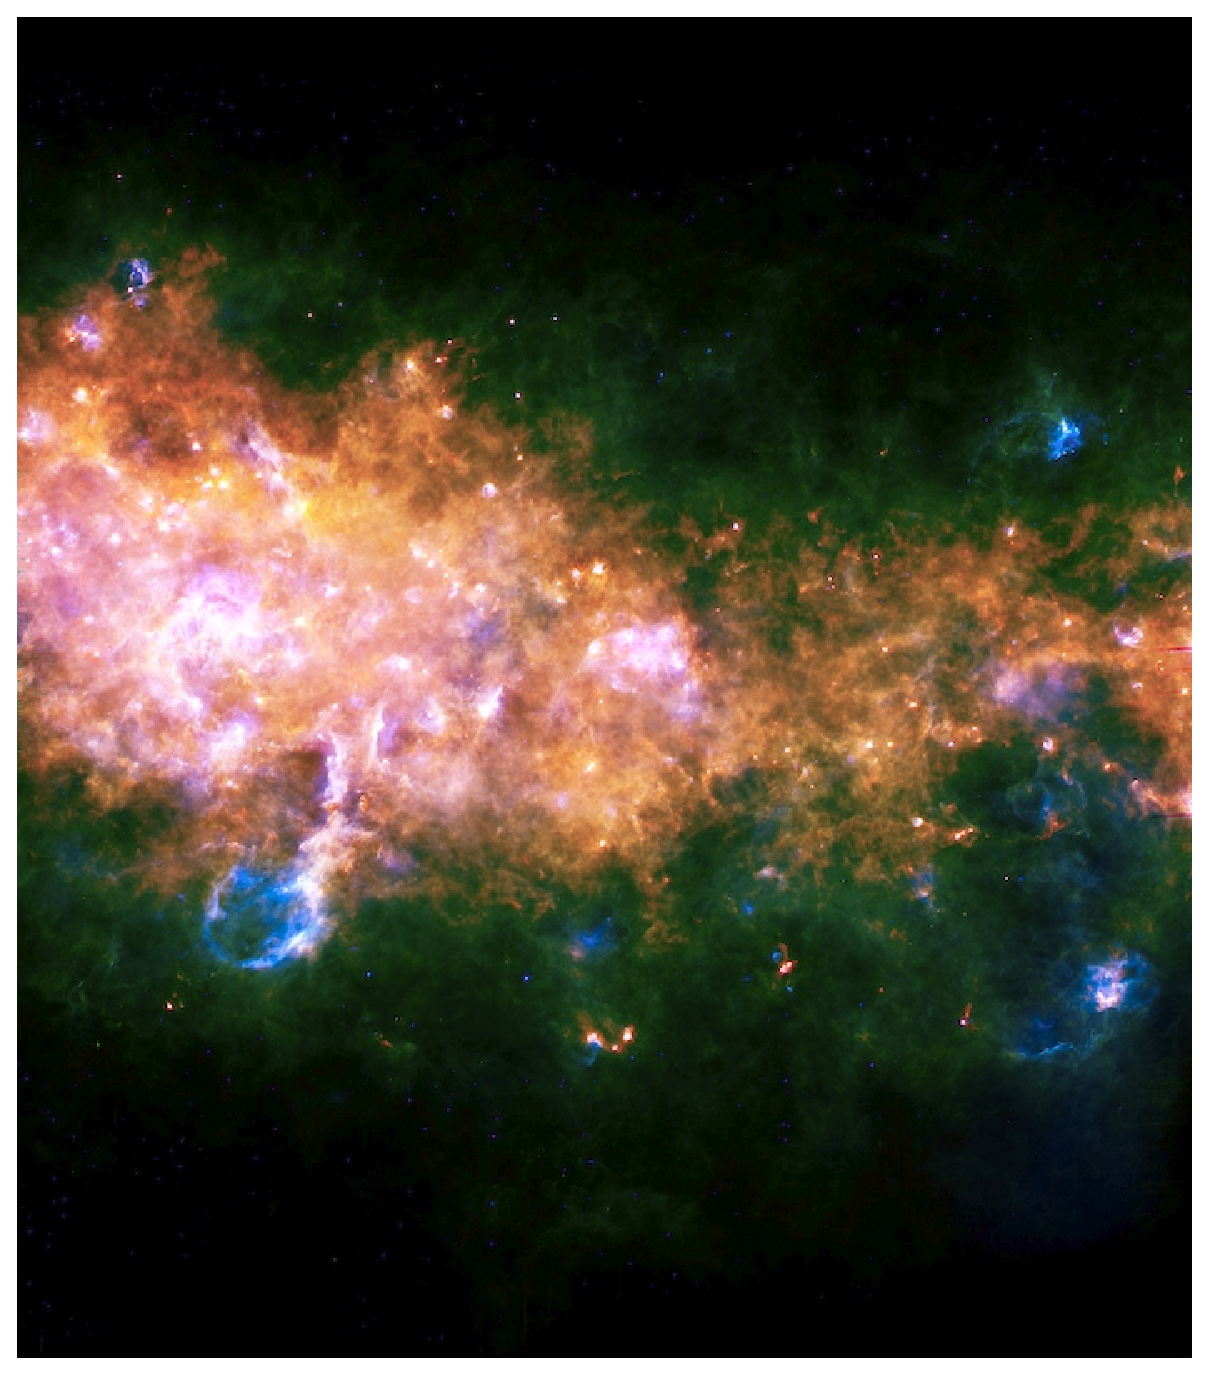
\includegraphics[width=0.382\textwidth]{Stellar_Gestation_and_Birth_in_the_Milky_Way.eps}
	%	\caption{Stern\-ent\-steh\-ungs\-ge\-biet im Ad\-ler\-ne\-bel. Auf\-ge\-nom\-men mit Her\-schel bei 70, 160 und 250$\mu$m im Dezember 2009.}
		% ($18^\text{h}46^\text{m}5.22^\text{s}$ / $+2^\circ 36'32.88"$)
	%	\vspace{-2em}
	%	\label{fig:starformingregion}
	%\end{wrapfigure}
	Auf den verschiedenen Beobachtungen lassen sich empirisch Theorien der Stern- und Planetenentstehung gründen. Der andere Weg führt ausgehend von etablierten allgemeinen Theorien über mathematische Herleitungen oder ``first--principles''--Simulationen zu Vorhersagen oder zum Nachvollzug der verschiedenen Phasen der Stern- und Planetenentstehung. Beide Wege sind nicht unabhängig voneinander sondern bilden vielmehr Abschnitte auf einem spiralförmigen Weg auf dem sich Empirie und Theorie abwechseln und durch Induktion und Deduktion gegenseitig eine bessere Ausgangslage schaffen.
	
	Im Bereich protoplanetarer Scheiben bildet Strahlungstransport den Teil der Theorie, der Vorhersagen über das Verhalten von Licht in einer vorgegebenen Anordnung von Materie macht. Strahlungstransport ist im Bereich protostellarer Scheiben somit einerseits wichtig für ein vollständiges Modell ihres Aufbaus, und andererseits wichtig, um ihr Aussehen vorherzusagen. Eine Simulation des Strahlungstransports erlaubt den Vergleich von Bildern aus Scheibenmodellen und mithilfe von Teleskopen aufgenommenen Bildern und stellt somit das direkte Bindeglied zwischen Theorie und Beobachtung dar.
	
	Wir leben dabei in einer spannenden Zeit, in der die aktuelle und kommende Generation von Großteleskopen auf der Erde und im Weltraum detailreichere Daten von protostellaren Scheiben aufnehmen als je zuvor. Dies stellt auch höhere Anforderungen an Strahlungstransportsimulationen, von denen feinere und genauere Bilder und Spektren gebraucht werden, um beim Vergleich mit Beobachtungsdaten von Nutzen zu sein.
	
	Dabei stellt sich häufig nicht das Problem, das Aussehen einer vorgegebenen Scheibenkonfiguration zu simulieren, sondern das inverse Problem --- nämlich aus gegebenen Beobachtungsdaten unter physikalischen Nebenbedingungen die wahrscheinlichste Materieanordnung zu finden, um die Beobachtung zu erklären. Das direkte Lösen dieses Problems ist im Allgemeinen nicht möglich. Daher ist der praktisch gegangene Ausweg das mehr oder weniger intelligente Raten von möglichst passenden Scheibenkonfigurationen, die nach einer Strahlungstransportsimulation mit den Beobachtungsdaten verglichen werden können. In dieser Situation ist eine effiziente Simulation umso nützlicher und unter Umständen entscheidend für den Unterschied zwischen dem Raten eines spezifischen Modells aufgrund einiger weniger Modellrechnungen und einer abdeckenden, statistisch signifikanten Schätzung der Modellparameter.
	
	Daher sollen in dieser Arbeit neue Ansätze zur effizienten Lösung des Strahlungstransportproblems vorgestellt, erprobt und diskutiert werden.
	
	\section{Ziele der Arbeit}
	In dieser Arbeit wird eine Pfadintegraldarstellung der Lösung des Strahlungstransportgleichung hergeleitet sowie dessen Nutzen für Monte--Carlo--Verfahren zur Lösung des Strahlungstransportproblems theoretisch und praktisch in Form eines Computerprogrammes gezeigt.
	
	\section{Übersicht}
	Wir fangen in Kapitel 2 mit einer Einführung des Strahlungstransportproblems anhand eines allgemeinen Teilchentransportproblems an, welches wir anschließend durch Spezialisierung der Teilchen auf Photonen auf die klassische Strahlungstransportgleichung zurückführen. Außerdem stellen wir einen allgemeinen Formalismus für Messungen des Strahlungsfeldes vor.
	
	In Kapitel 3 überführen wir die klassische Strahlungstransportgleichung über den Umweg einer Integraldarstellung in eine Operatorform, in der das Problem anschaulich und formal leicht lösbar ist. Die gewonnene Lösung stellen wir dann als Integral über den Raum aller möglichen Lichtpfade dar.
	
	In Kapitel 4 beschäftigen wir uns mit dem Problem der numerischen Integration und den Vor- und Nachteilen der Monte--Carlo--Integration im Vergleich zu klassischen numerischen Quadraturverfahren.
	
	In Kapitel 5 stellen wir ein weiteres Monte--Carlo--Verfahren vor, mit dem sich aus beliebigen statistischen Verteilungen Stichproben erzeugen lassen und erklären, wozu dies im Zusammenhang mit der Lösung des Strahlungstransportproblems nützlich ist.
	
	In Kapitel 6 führen wir die bis dahin behandelten Themen Strahlungstransport und Monte--Carlo--Verfahren zusammen. Wir zeigen, wie sich die in Kapitel 3 hergeleitete Pfadintegrallösung des Strahlungstransportproblems als Integrationsproblem darstellen lässt, auf die unsere Monte--Carlo--Integrationsverfahren aus Kapitel 4 direkt anwendbar sind. Ergänzend dazu stellen wir Methoden vor, um die Konvergenz der Integration durch eine gehäuftere Berücksichtigung der für den Strahlungstransport wesentlichen Pfade zu verbessern.
	
	In Kapitel 7 stellen wir das Programm \pirate vor, in dem viele der vorgestellten Ideen implementiert sind.
	
	In Kapitel 8 vergleichen wir dann die Ergebnisse und die Geschwindigkeit von \pirate mit dem Referenzprogramm \texttt{MC3D}.
	
	Schließlich fassen wir in Kapitel 9 die Arbeit zusammen und geben einen Ausblick, wie die vorgestellten Ideen und das Programm \pirate weiterentwickelt und eingesetzt werden können.
	
	\vfill
	\pagebreak
	\section{Nomenklatur}\label{subsec:nomenklatur}
	Im folgenden Text werden die in Tabelle \ref{tab:nomenklatur} angegebenen Schreibweisen benutzt.

	\begin{table}
		\caption{Nomenklatur}
		\begin{center}
		\begin{tabular}{rll}
			Schreibweise & Bedeutung & Einheit \\
			\hline
			$\kappa(\location{r})$ & Volumenabsorptionsquerschnitt am Ort $\location{r}$& $\left[\text{m}^2/\text{m}^3\right]$ \\
			$\sigma(\location{r})$ & Volumenstreuquerschnitt am Ort $\location{r}$ & $\left[\text{m}^2/\text{m}^3\right]$ \\
			$\xi(\location{r})$ & Volumenextinktionsquerschnitt am Ort $\location{r}$ & $\left[\text{m}^2/\text{m}^3\right]$ \\
			$\varepsilon(\location{r},\omega)$ & Volumenemissivität am Ort $\location{r}$ in Richtung $\omega$ & $\left[\text{W}/(\text{m}^3\,\text{sr})\right]$ \\
			$I(\location{r},\omega)$ & Intensität am Ort $\location{r}$ in Richtung $\omega$& $\left[\text{W}/(\text{m}^2\,\text{sr})\right]$ \\
			$W(\location{r},\omega)$ & Sensitivität am Ort $\location{r}$ in Richtung $\omega$ & $\left[(\text{m}^2\,\text{sr})/\text{W}\right]$ \\
			$k(\location{r},\omega',\omega)$ & Phasenfunktion am Ort $\location{r}$ für ein Teilchen, & $\left[1/\text{sr}\right]$ \\
				&das sich vor der Streuung in Richtung $\omega'$&\\
				&und nach der Streuung in Richtung $\omega$ bewegt& \\
			$\tau(\location{r}_i,\location{r}_j)$ & Optische Tiefe zwischen $\location{r}_i$ und $\location{r}_j$ & \\
			$\varepsilon_{(i,j)}$ & Emissivität am Ort $\location{r}_i$ in Richtung $\normalized{\location{r}_j-\location{r}_i}$ & \\
			$W_{(i,j)}$ & Sensitivität am Ort $\location{r}_j$ für Strahlung in Richtung $\normalized{\location{r}_j-\location{r}_i}$ & \\
			$\scatter{i}$ & Produkt aus Volumenstreuquerschnitt und&\\
			  & Streuphasenfunktion am Ort $\location{r}_i$ für ein aus Richtung $\location{r}_{i-1}$&\\ 
				&kommendes und in Richtung $\location{r}_{i+1}$ gestreutes Teilchen&\\
				&(äquivalent zu $\sigma(\location{r}_i)k(\location{r}_i,\normalized{\location{r}_i-\location{r}_{i-1}},\normalized{\location{r}_{i+1}-\location{r}_i})$)& \\
			$\propagate{i}{j}$ & Produkt aus Abschwächungsfaktor aufgrund optischer Tiefe&\\
			  &und geometrischem Verdünnungsfaktor zwischen $\location{r}_i$ und $\location{r}_{j}$&\\ 
				&(äquivalent zu $\frac{e^{-\tau(\location{r}_{i},\location{r}_j)}}{\|\location{r}_j-\location{r}_{i}\|^2}$)& \\
			
		\end{tabular}
		\end{center}
		\label{tab:nomenklatur}
	\end{table}
